\vspace{-0.2cm}
\section{Background on Hardware Accelerators}
\vspace{-0.2cm}
\label{sec:accelerator_background}
The goal of specialized hardware accelerators---Google TPUs~\citep{jouppi2017datacenter,edgetpu:arxiv:2020}, Nvidia GPUs~\citep{nvidia}, GraphCore~\citep{graphcore}---is to improve the performance of specific applications, such as machine learning models. To design such accelerators, architects typically create a parameterized design and sweep over parameters using simulation.

\niparagraph{Target hardware accelerators.}
%
Our primary evaluation uses an industry-grade and highly parameterized template-based accelerator following prior work~\citep{yazdanbakhsh2021evaluation}.
%
This template enables architects to determine the organization of various components, such as compute units, memory cells, memory, etc., by searching for these configurations in a discrete design space. Some ML applications may have large memory requirements (e.g., large language models~\citep{brown2020language}) demanding sufficient on-chip memory resources, while others may benefit from more compute blocks. The hardware design workflow directly selects the values of these parameters.
%
In addition to this accelerator and to further show the generality of our method to other accelerator design problems, we evaluate two distinct dataflow accelerators with different search spaces, namely NVDLA-style~\citep{nvdla} and ShiDianNao-style~\citep{shidiannao} from~\citet{kao2020confuciux} (See Section~\ref{sec:eval} and Appendix~\ref{sec:dla_shi_fast} for a detailed discussion; See Table~\ref{table:dla_shi} for results).

\begin{wrapfigure}{r}{0.47\textwidth}
    \centering
    \vspace{-0.1in}
    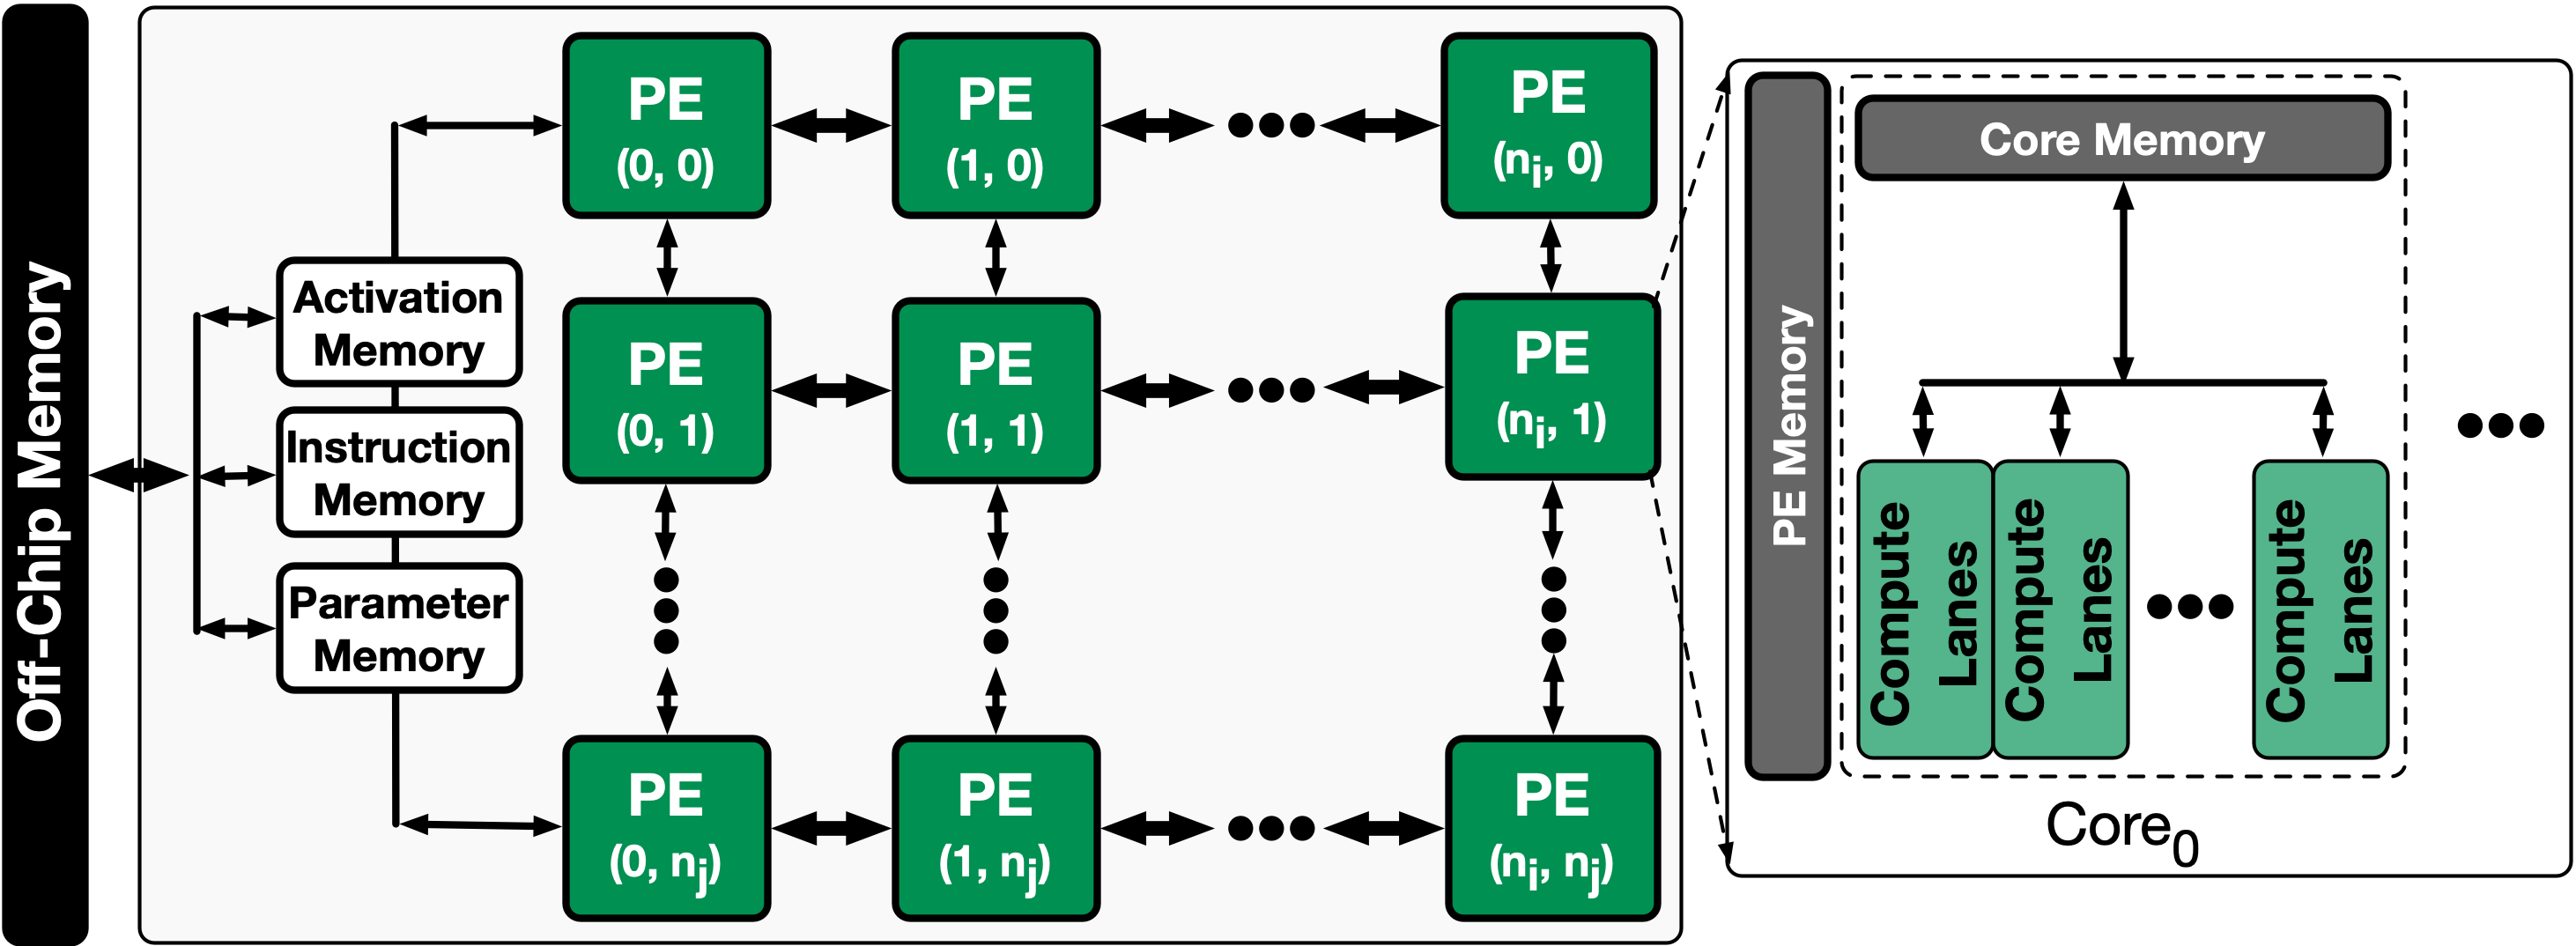
\includegraphics[width=0.98\linewidth]{chapters/prime/figs/accelerator/template-accel.png}
    \vspace{-0.1cm}
    \caption{An industry-level machine learning accelerator~\cite{yazdanbakhsh2021evaluation}.}
    \label{fig:template_accel}
    \vspace{-0.5cm}
    \label{fig:accels}
\end{wrapfigure} 

\niparagraph{How does an accelerator work?}
%
We briefly explain the computation flow on our template-based accelerators (Figure~\ref{fig:template_accel}) and refer the readers to Appendix~\ref{sec:dla_shi_fast} for details on other accelerators. This template-based accelerator is a 2D array of processing elements (PEs). Each PE is capable of performing matrix multiplications in a single instruction multiple data (SIMD) paradigm~\citep{simd}. A controller orchestrates the data transfer (both activations and model parameters) between off-chip DRAM memory and the on-chip buffers and also reads in and manages the instructions (e.g. convolution, pooling, etc.) for execution. The computation stages on such accelerators start by sending a set of activations to the compute lanes, executing them in SIMD manner, and either storing the partial computation results or offloading them back into off-chip memory. Compared to prior works~\citep{hegdemind,shidiannao,kao2020confuciux}, this parameterization is unique---it includes multiple compute lanes per each PE and enables SIMD execution model within each compute lane---and yields a distinct accelerator search space accompanied by an end-to-end simulation framework. 
% More details in Appendix~\ref{sec:dla_shi_fast}.